%!TEX root=../GaugeCNNTheory.tex


\subsection{تقریب‌های بیست‌وجهی از \lr{CNN}های کروی}
\label{sec:spherical_CNNs_icosahedral}

کره $S^2$ در علوم محاسباتی معمولاً با اجسام افلاطونی، یعنی چندوجهی‌های منتظم محدب، تقریب زده می‌شود.
در زمینه یادگیری عمیق، علاقه بیشتر بر روی بیست‌وجهی (icosahedron)، شکل~\ref{fig:ico_neighborhoods}، متمرکز شده است، که در میان اجسام افلاطونی، نزدیک‌ترین تقریب به کره است~\cite{schroder1995spherical}.
در حالی که هندسه ریمانی کره فقط تقریب زده می‌شود، اجسام افلاطونی این مزیت را دارند که تکه‌ای-تخت هستند و مش‌های منظمی را می‌پذیرند.
این ویژگی‌ها امکان استفاده از روال‌های کانولوشن مسطح را فراهم می‌کنند، که از نظر محاسباتی بهینه‌تر از روش‌های دو بخش قبل هستند.
این بخش به بحث در مورد \lr{CNN}های بیست‌وجهی از~\cite{liu2018icoAltAz}، \cite{zhang2019orientation} و~\cite{gaugeIco2019} می‌پردازد، که به ترتیب بر $G$-ساختارهای نشان داده شده در شکل‌های~\ref{fig:G_structure_ico_1}، \ref{fig:G_structure_ico_2} و~\ref{fig:G_structure_ico_3} تکیه دارند.
قبل از پرداختن به پیاده‌سازی‌های آنها بر حسب اطلسی از چارت‌های آفين در شکل~\ref{fig:ico_cutting}،
ما جزئیات بیشتری در مورد هندسه بیست‌وجهی و $G$-ساختارهای در نظر گرفته شده ارائه می‌دهیم.


\begin{figure}
    \centering
    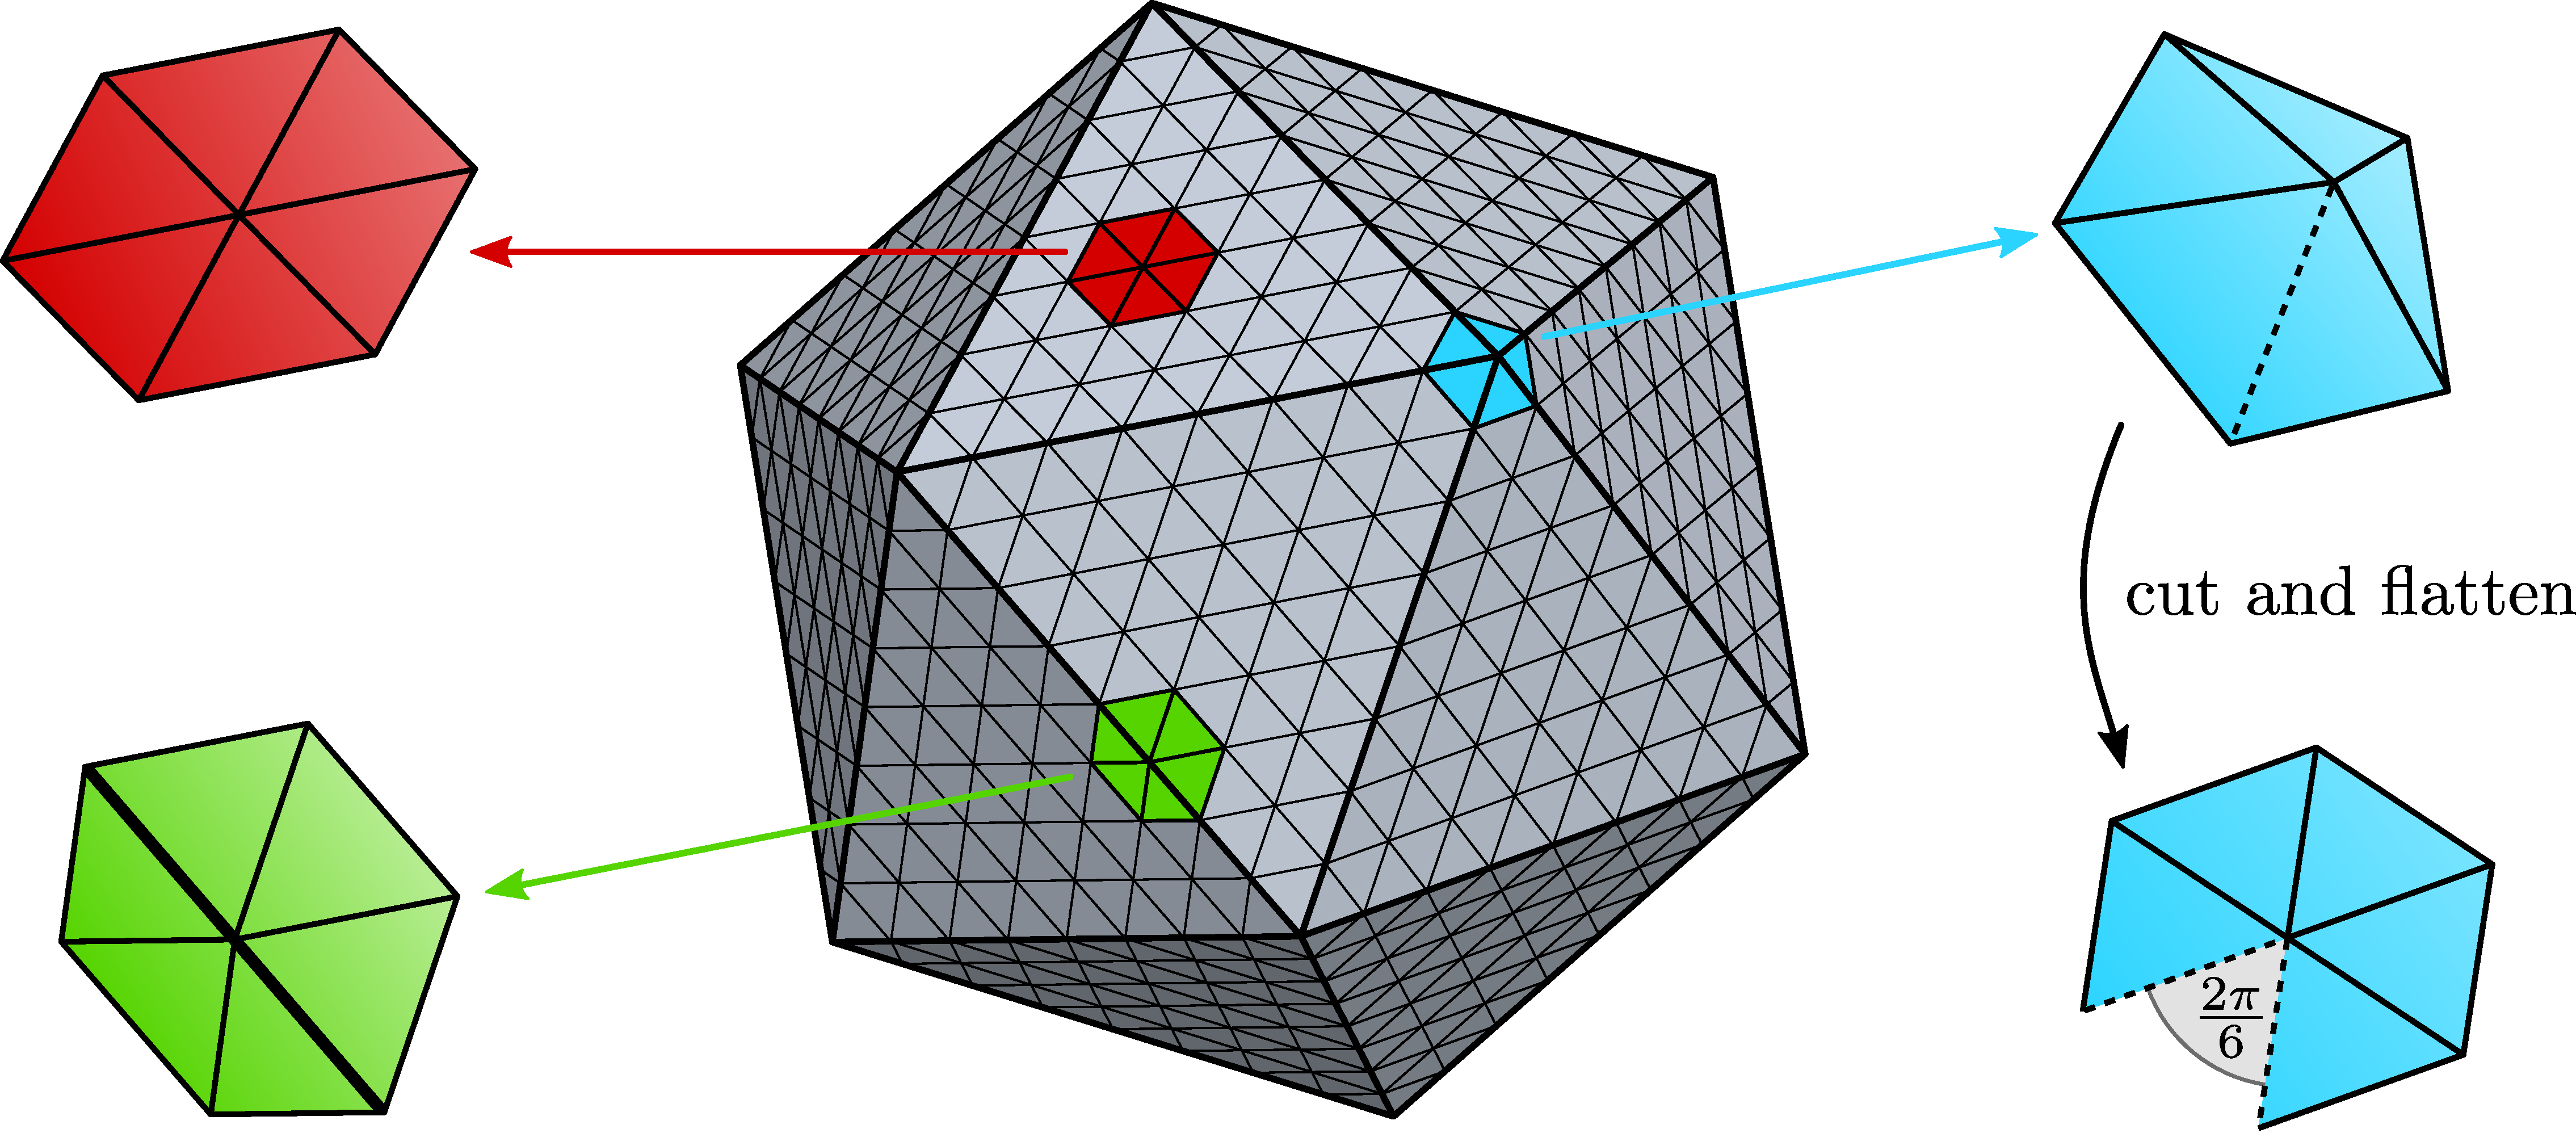
\includegraphics[width=.8\textwidth]{figures/icosahedron_neighborhoods.pdf}
    \vspace*{1ex}
    \caption{\small
        بیست‌وجهی یک جسم افلاطونی است که در \cite{liu2018icoAltAz,gaugeIco2019,zhang2019orientation} به عنوان یک تقریب تکه‌ای-تخت از هندسه کروی استفاده می‌شود.
        این جسم از ۱۲ رأس، ۲۰ وجه مثلثی متساوی‌الاضلاع و ۳۰ یال تشکیل شده است.
        این جسم یک شبکه نمونه‌برداری منظم را می‌پذیرد، که با تقسیم مکرر هر مثلث به چهار مثلث کوچکتر ساخته می‌شود.
        پس از $r$ تکرار، این رویه منجر به یک شبکه با ${5\mkern-1mu\cdot\mkern-1mu 2^{2r+1} + 2}$ رأس می‌شود.
        سه تکه برجسته شده، هندسه کیفی متفاوت همسایگی‌ها را حول رئوس روی وجوه (قرمز)، یال‌ها (سبز) و رئوس بیست‌وجهی (آبی) نشان می‌دهند.
        همسایگی قرمز به وضوح تخت است.
        در حالی که همسایگی سبز در فضای جایگذاری خمیده است، انحنای گاوسی ذاتی آن دوباره صفر است.
        این واقعیت در این امر منعکس می‌شود که می‌توان آن را به صورت ایزومتریک (یعنی بدون برش) پهن کرد و به طور معادل، انتقال لوی-چیویتا در امتداد یک مسیر بسته حول گره مرکزی، نگاشت همانی است.
        همسایگی آبی باید در امتداد یک یال بریده شود تا بتوان آن را پهن کرد.
        نقص زاویه، یعنی زاویه‌ای که برش هنگام پهن کردن نوک تیز باز می‌شود، برابر با~$\frac{2\pi}{6}$ است.
        هنگامی که یک بردار یک بار حول رأس مرکزی همسایگی به صورت موازی منتقل می‌شود، به اندازه این نقص زاویه می‌چرخد.
        به جای داشتن انحنای گاوسی مثبت ثابت مانند کره $S^2$، انحنای بیست‌وجهی در رئوس آن متمرکز (تکین) است و در همه جای دیگر صفر است.
    }
    \label{fig:ico_neighborhoods}
\end{figure}


\paragraph{هندسه‌ی بیست‌وجهی:}
بیست‌وجهی یک منیفلد دوبعدی گسسته است که از ۲۰ وجه مثلثی متساوی‌الاضلاع، ۱۲ رأس و ۳۰ یال تشکیل شده است.
همانند کره ۲-بعدی، ما بیست‌وجهی را به عنوان جایگذاری شده در $\R^3$ تعریف می‌کنیم، که از آن متریک جایگذاری را در معادله~\eqref{eq:spherical_embedding_metric_explicit} به ارث می‌برد.
فضاهای مماس جایگذاری شده $\TpM \subset \R^3$ روی وجوه در اینجا به گونه‌ای تعریف می‌شوند که نرمال‌های آنها با نرمال‌های وجوه منطبق باشند.
فضاهای مماس روی رئوس و یال‌ها را می‌توان از طریق میانگین نرمال‌های وجوه مجاور تعریف کرد، همانطور که در بخش بعدی~\ref{sec:instantiations_mesh} مورد بحث قرار می‌گیرد.
با این حال، از آنجا که ما میدان‌های ویژگی را به عنوان نمونه‌برداری شده روی وجوه بیست‌وجهی (که تقریباً همه جا است) در نظر می‌گیریم، از این انتخاب مستقل هستیم.
با فرض اتصال لوی-چیویتا، انتقال موازی بردارهای مماس روی وجوه به گونه‌ای عمل می‌کند که آنها را در فضای جایگذاری~$\R^3$ موازی نگه دارد.
هنگامی که بردارهای مماس از روی یک یال به صورت موازی منتقل می‌شوند، زاویه یکسانی را نسبت به یال در هر دو طرف حفظ می‌کنند -- این انتقال را می‌توان به طور شهودی به این صورت تصور کرد که ۱) دو وجه مجاور را پهن کرده، ۲) بردار را روی یال مانند حالت معمول در یک فضای اقلیدسی دوبعدی منتقل کرده، و ۳) دو وجه را به جایگذاری اصلی خود بازگردانیم؛ به شکل~\ref{fig:transport_mesh} و \cite{craneDiscreteDifferentialGeometry2014} مراجعه کنید.
بنابراین ژئودزیک‌ها در $\R^3$ تکه‌ای-خطی هستند و از یال‌ها به گونه‌ای عبور می‌کنند که زاویه خروج آنها برابر با زاویه ورودشان باشد.
بنابراین نگاشت‌های نمایی $\exp_p(v)$ به راحتی با دنبال کردن یک مسیر تکه‌ای-ثابت برای فاصله‌ای برابر با $\lVert v\rVert$ محاسبه می‌شوند.
در عمل، نویسندگان~\cite{liu2018icoAltAz,gaugeIco2019,zhang2019orientation} میدان‌های ویژگی را روی یک مش منظم نمونه‌برداری می‌کنند و فقط آن دسته از بردارهای مماس را در نظر می‌گیرند که به رئوس مش همسایه نگاشت می‌یابند.


شکل~\ref{fig:ico_neighborhoods} همسایگی‌های دیسک‌مانند را حول نقاط نمونه روی وجوه (قرمز)، یال‌ها (سبز) و رئوس (آبی) بیست‌وجهی نشان می‌دهد.
همسایگی قرمز کاملاً در داخل یک وجه قرار دارد و بنابراین تخت است.
همسایگی سبز در فضای جایگذاری خمیده است، با این حال، انحنای ذاتی (ریمانی یا گاوسی) آن هنوز صفر است زیرا انتقال لوی-چیویتا بردارها یک بار حول رأس مرکزی، آنها را همانطور که هستند حفظ می‌کند.
اینکه این مورد برقرار است معادل این واقعیت است که همسایگی سبز را می‌توان به صورت ایزومتریک پهن کرد، یعنی بدون کشش یا برش آن.
این پهن‌کردن ایزومتریک برای نوع آبی همسایگی‌ها حول رئوس ممکن نیست، که برای پهن شدن باید در یکی از یال‌ها بریده شوند.
با ساخته شدن از پنج مثلث متساوی‌الاضلاع، نوک تیز پهن شده یک نقص زاویه~$\frac{2\pi}{6}$ را نشان می‌دهد.
هولونومی هر مسیر بسته حول هر رأس (منفرد)، یعنی زاویه بین یک بردار دلخواه و انتقال آن یک بار حول حلقه، دقیقاً با این نقص زاویه داده می‌شود.
در کل، این نتایج دلالت بر این دارند که انحنای گاوسی (گسسته) بیست‌وجهی در همه جا به جز در رئوس صفر است، جایی که با هولونومی $\frac{2\pi}{6}$ تکین است.
هندسه ساده بیست‌وجهی اجازه می‌دهد تا آن را باز کرده و به صورت سراسری پهن کرد، همانطور که در شکل~\ref{fig:ico_cutting} به تصویر کشیده شده است، که در~\cite{liu2018icoAltAz,gaugeIco2019,zhang2019orientation} برای یک پیاده‌سازی کارآمد از کانولوشن‌های $\GM$ بیست‌وجهی استفاده شد.


گروه ایزومتری کامل بیست‌وجهی $\IsomM = \operatorname{I}_h \leq \OO3$ متناهی است و از ۱۲۰ عضو تشکیل شده است.
می‌توان آن را به عنوان حاصلضرب مستقیم $\operatorname{I} \times \Flip$ از زیرگروه بازتاب‌ها $\Flip$ و زیرگروه ایزومتری‌های حافظ جهت $\IsomplusM = \operatorname{I} \leq \SO3$ که شامل ۶۰ دوران است، ساخت.
هر رأس~$p$ توسط پنج دوران گسسته حول محور گذرنده از $p$ و رأس متقابل آن پایدار می‌شود، که گروه دوری~$\operatorname{C}_5 \leq \SO2$ را تشکیل می‌دهند.
رأس~$p$ علاوه بر این توسط بازتاب‌ها نسبت به صفحه تعریف شده توسط محور دوران و هر یال خروجی از~$p$ پایدار می‌شود، به طوری که زیرگروه پایدارساز کامل آن با گروه دووجهی $\Stab{p} = \operatorname{D}_5 \leq \OO2$ داده می‌شود.
هموردایی کانولوشن‌های $\GM$ بیست‌وجهی نسبت به گروه‌های ایزومتری $\operatorname{I}_h$, $\operatorname{I}$, $\operatorname{D}_5$ یا $\operatorname{C}_5$ در~\cite{gaugeIco2019} نشان داده شده است که هموردایی کامل $\OO3$, $\SO3$, $\OO2$ یا $\SO2$ \lr{CNN}های کروی را به خوبی تقریب می‌زند هنگامی که از افزایش داده دورانی پیوسته استفاده شود.%
\footnote{
	این در~\cite{gaugeIco2019} به صورت تجربی برای $\operatorname{I} \leq \SO3$ نشان داده شده است.
	اینکه این نتیجه به $\operatorname{I}_h \leq \OO3$ تعمیم می‌یابد، روشن است زیرا گروه‌ها فقط در بازتاب‌ها متفاوت هستند، که کانولوشن‌های $\GM$ بیست‌وجهی را می‌توان نسبت به آنها دقیقاً هموردا ساخت.
	این علاوه بر این برای $\operatorname{D}_5 \leq \OO2$ و $\operatorname{C}_5 \leq \SO2$ نیز برقرار است، زیرا اینها زیرگروه‌هایی از $\operatorname{I}_h \leq \OO3$ هستند.
}


\begin{figure*}
    \centering
    \begin{subfigure}[b]{0.31\textwidth}
        \centering
        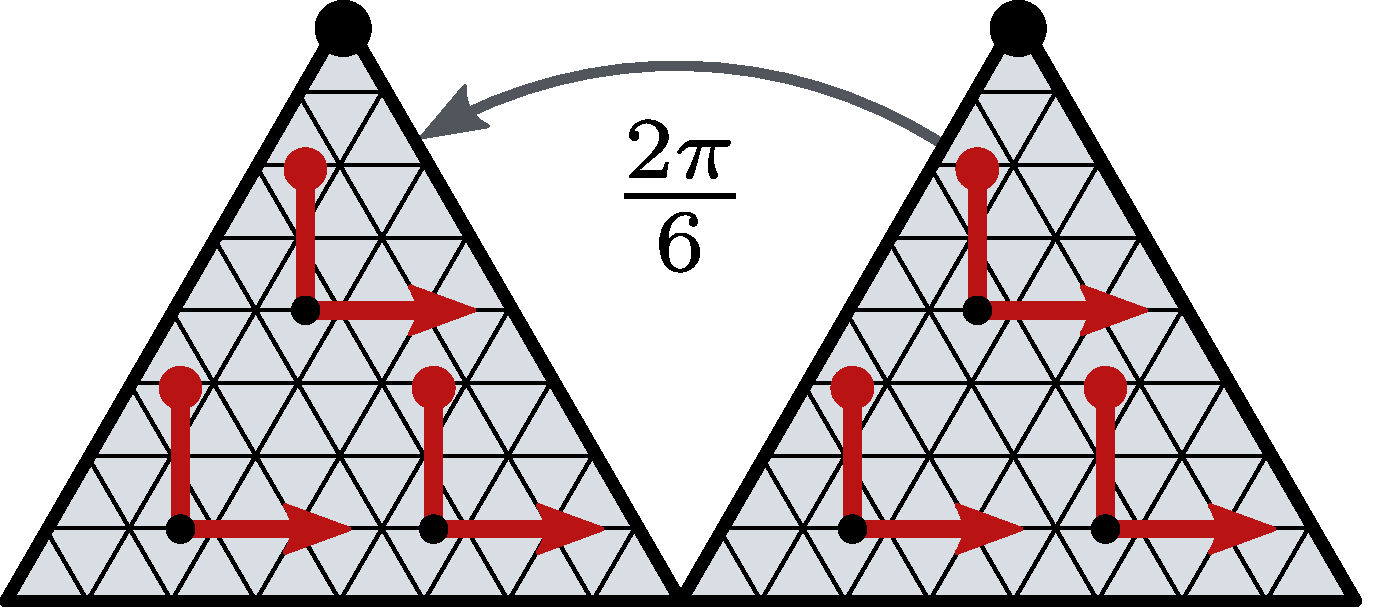
\includegraphics[width=1.\textwidth]{figures/icosahedron_G_structure_1.pdf}
        \vspace*{-6pt}
        \captionsetup{width=.9\textwidth}
        \caption{\small
            $\{e\}$-ساختار بیست‌وجهی تراز-شده-با-شبکه توسط \citet{liu2018icoAltAz}.
        }
        \label{fig:G_structure_ico_1}
    \end{subfigure}
    \hfill
    \begin{subfigure}[b]{0.31\textwidth}
        \centering
        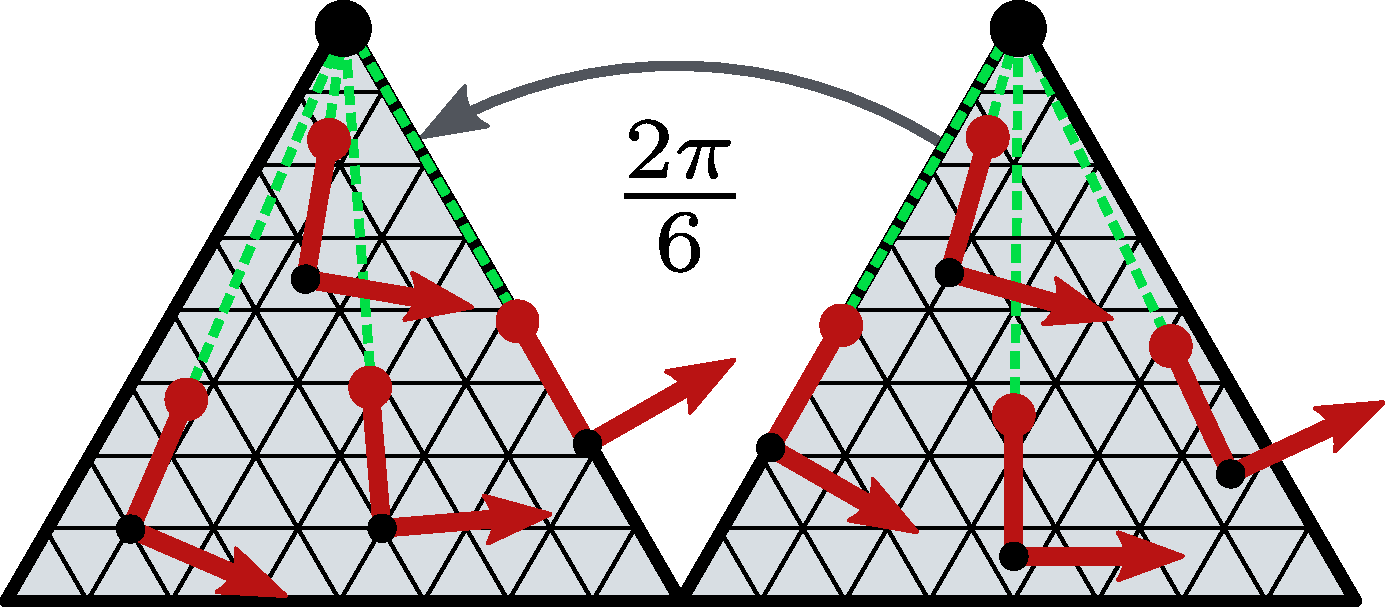
\includegraphics[width=1.\textwidth]{figures/icosahedron_G_structure_2.pdf}
        \vspace*{-6pt}
        \captionsetup{width=.9\textwidth}
        \caption{\small
            $\{e\}$-ساختار بیست‌وجهی تراز-شده-به-شمال توسط \citet{zhang2019orientation}.
        }
        \label{fig:G_structure_ico_2}
    \end{subfigure}
    \hfill
    \begin{subfigure}[b]{0.31\textwidth}
        \centering
        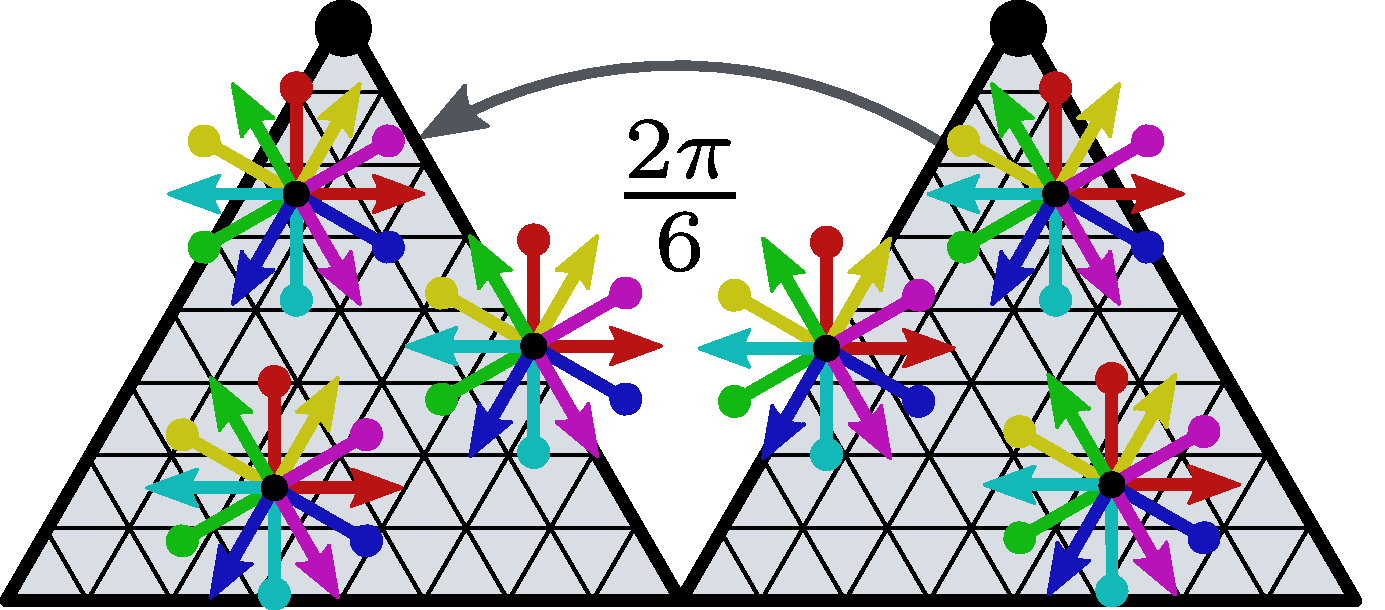
\includegraphics[width=1.\textwidth]{figures/icosahedron_G_structure_3.pdf}
        \vspace*{-6pt}
        \captionsetup{width=.9\textwidth}
        \caption{\small
            $\operatorname{C}_6$-ساختار بیست‌وجهی تراز-شده-با-شبکه توسط \citet{gaugeIco2019}.
        }
        \label{fig:G_structure_ico_3}
    \end{subfigure}
    \caption{\small
        ایده مفهومی $G$-ساختارهای فرض شده در~\cite{liu2018icoAltAz,zhang2019orientation,gaugeIco2019}.
        به دلیل محدودیت فضا، فقط دو وجه مجاور کنار قطب شمال از بیست‌وجهی پهن شده (شکل~\ref{fig:ico_cutting}) نشان داده شده است.
        $\{e\}$-ساختار در شکل~\ref{fig:G_structure_ico_1} با تراز کردن تمام چارچوب‌ها در امتداد یال‌های «افقی» وجوه (با فرض عمودی بودن محور قطبی) تعریف می‌شود.
        شکل~\ref{fig:G_structure_ico_2} یک $\{e\}$-ساختار جایگزین را نشان می‌دهد که چارچوب‌های آن به سمت قطب شمال تراز شده‌اند.
        این ساختار بر خلاف $\{e\}$-ساختار قبلی پیوسته است زیرا چارچوب‌ها روی یال‌های بریده شده هنگام چسباندن مجدد یال‌ها به یکدیگر منطبق می‌شوند.
        $\operatorname{C}_6$-ساختار در شکل~\ref{fig:G_structure_ico_3} با افزودن چارچوب‌هایی که با مضرب‌هایی از $\frac{2\pi}{6}$ چرخانده شده‌اند به $\{e\}$-ساختار از شکل~\ref{fig:G_structure_ico_1} ساخته می‌شود.
        از آنجا که این زاویه با نقص زاویه در یال‌های بریده شده برابر است، $\operatorname{C}_6$-ساختار تعریف شده به این ترتیب هموار (پیوسته) است.
        توجه داشته باشید که این دو $\{e\}$-ساختار با انتقال لوی-چیویتا ناسازگار هستند (یعنی تحت آن بسته نیستند) اما یک اتصال بدیهی جایگزین را القا می‌کنند.
        $\operatorname{C}_6$-ساختار، در مقابل، با انتقال لوی-چیویتا سازگار است.
    }
    \label{fig:G_structures_ico}
\end{figure*}


\paragraph{$G$-ساختارهای بیست‌وجهی:}
کانولوشن‌های $\GM$ بیست‌وجهی توسط~\citet{liu2018icoAltAz} و~\citet{zhang2019orientation} (به طور ضمنی) $\{e\}$-ساختارها را فرض می‌کنند، در حالی که مدل~\citet{gaugeIco2019} یک $\operatorname{C}_6$-ساختار را فرض می‌کند.
شکل~\ref{fig:G_structures_ico} ایده پشت این $G$-ساختارها را به تصویر می‌کشد، که در سه پاراگراف بعدی با جزئیات بیشتری توضیح می‌دهیم.


$\{e\}$-ساختار توسط~\citet{liu2018icoAltAz} که در شکل~\ref{fig:G_structure_ico_1} نشان داده شده است، با تراز کردن اولین محورهای چارچوب در امتداد یال‌های «افقی» وجوه مثلثی متناظر تعریف می‌شود.
هنگام پهن کردن بیست‌وجهی به یک صفحه همانطور که در شکل~\ref{fig:ico_cutting} نشان داده شده است، تمام چارچوب‌های این $\{e\}$-ساختار در این صفحه موازی هستند، که پیاده‌سازی کانولوشن‌های $\GM$ متناظر را بسیار ساده می‌کند.
طبق معمول، $\{e\}$-ساختار یک اتصال بدیهی یکتا را مشخص می‌کند که ویژگی‌ها مطابق آن منتقل می‌شوند.
این اتصال بدیهی در داخل وجوه، روی یال‌هایی که در شکل~\ref{fig:ico_cutting} بریده نشده‌اند و روی یال بریده شده ارغوانی با اتصال لوی-چیویتا منطبق است.
با این حال، انتقال آن از روی یال‌های بریده شده باقی‌مانده با انتقال لوی-چیویتا متفاوت است زیرا چارچوب‌های $\{e\}$-ساختار در آنجا به طور ناپیوسته به اندازه زاویه~$\frac{2\pi}{6}$ می‌چرخند.
از آنجا که $\{e\}$-ساختار توسط دوران‌ها در $\operatorname{C}_5$ حول محور قطبی حفظ می‌شود، کانولوشن‌های $\GM$ آن تقریباً $\SO2$-هموردا هستند، یعنی مدل‌های بخش قبلی~\ref{sec:spherical_CNNs_azimuthal_equivariant} را تقریب می‌زنند.
با این حال، $\{e\}$-ساختار -- و بنابراین استنتاج شبکه -- روی یال‌های با نقص زاویه غیرصفر \emph{ناپیوسته} است.
علاوه بر این، چارچوب‌های مرجع دقیقاً به سمت قطب شمال اشاره نمی‌کنند، همانطور که برای $\{e\}$-ساختار کروی از بخش~\ref{sec:spherical_CNNs_azimuthal_equivariant} و شکل~\ref{fig:G_structure_S2_2} صادق است.


\citet{zhang2019orientation} پیشنهاد می‌کنند که دو مشکل اخیر را با کار کردن با $\{e\}$-ساختار در شکل~\ref{fig:G_structure_ico_2} حل کنند.
این ساختار به گونه‌ای تعریف شده است که چارچوب‌ها دقیقاً در امتداد تصویر محور قطبی روی وجوه، یعنی به سمت قطب شمال، اشاره می‌کنند.
این $\{e\}$-ساختار در همه جا به جز در قطب‌های شمال و جنوب پیوسته است.%
\footnote{
	برای دیدن این، تصور کنید که یال بریده شده در شکل~\ref{fig:G_structure_ico_2} را دوباره به هم بچسبانید:
	چارچوب‌های روی نیمه چپ و راست یال سپس با هم منطبق می‌شوند، که این مورد در شکل~\ref{fig:G_structure_ico_1} صادق نیست.
}
این ساختار به این معنا تقریب بهتری از $\{e\}$-ساختار کروی از شکل~\ref{fig:G_structure_S2_2} است.
$\{e\}$-ساختار دوباره یک اتصال بدیهی یکتا را القا می‌کند.
انتقال آن با انتقال لوی-چیویتا روی یال‌ها منطبق است، با این حال، هنگام انتقال روی وجوه با آن متفاوت است زیرا بردارها را به آرامی همراه با چارچوب‌ها می‌چرخاند.
مانند $\{e\}$-ساختار دیگر، این میدان چارچوب تحت دوران‌های سمتی در $\operatorname{C}_5$ ناوردا است و بنابراین \lr{CNN}های کروی هموردای دوران سمتی را تقریب می‌زند.


$\operatorname{C}_6$-ساختار در شکل~\ref{fig:G_structure_ico_3} توسط~\citet{gaugeIco2019} با افزودن چارچوب‌هایی که با مضرب‌هایی از $\frac{2\pi}{6}$ چرخانده شده‌اند به چارچوب‌های $\{e\}$-ساختار از شکل~\ref{fig:G_structure_ico_1} تعریف می‌شود.
این ساختار به وضوح پیوسته است زیرا زوایای بین مجموعه چارچوب‌های مرجح در هر نقطه دقیقاً برابر با نقص‌های زاویه در یال‌های بریده شده است.
این ساختار بر خلاف دو $\{e\}$-ساختار قبلی با انتقال لوی-چیویتا سازگار است زیرا گروه ساختاری $\operatorname{C}_6$ با گروه هولونومی بیست‌وجهی منطبق است.
$\operatorname{C}_6$-ساختار علاوه بر این تحت عمل ایزومتری‌های حافظ جهت بیست‌وجهی $\operatorname{I}$ حفظ می‌شود.
بنابراین کانولوشن‌های $\GM$ روی این $\operatorname{C}_6$-ساختار، \lr{CNN}های کروی کاملاً هموردای دورانی $\SO3$ را از بخش~\ref{sec:spherical_CNNs_fully_equivariant} تقریب می‌زنند.

\begin{figure}
    \centering
    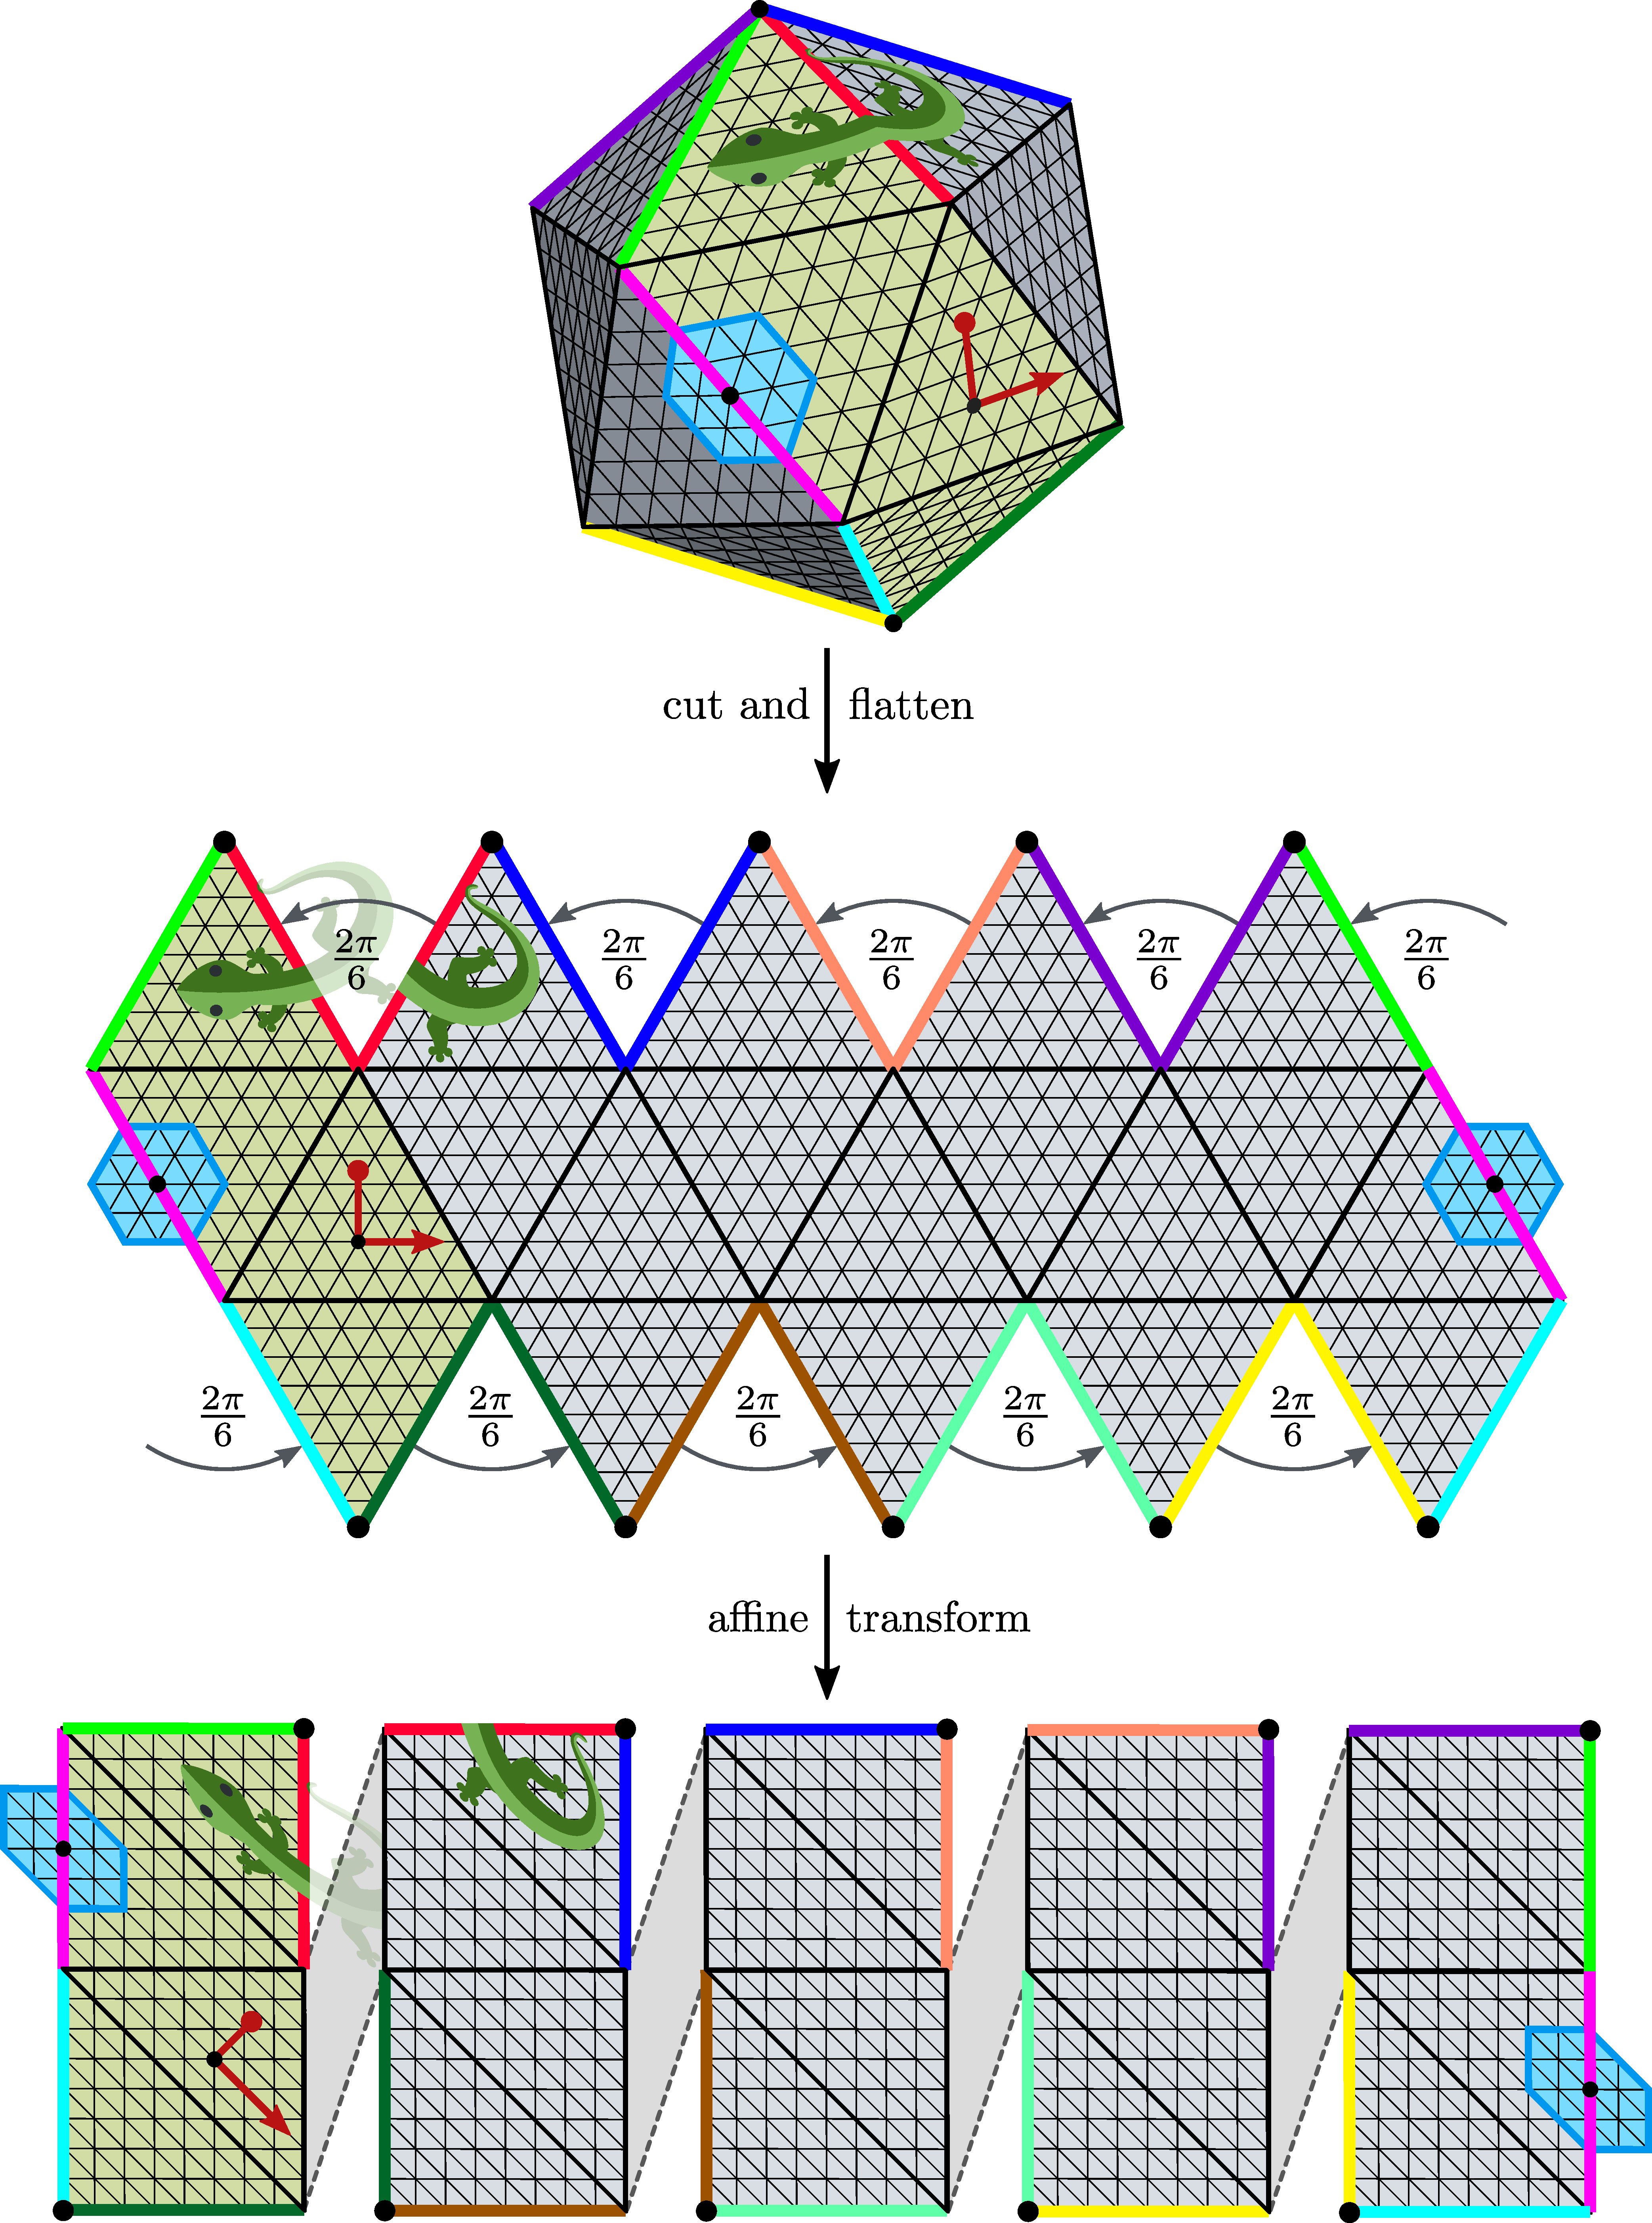
\includegraphics[width=.9\textwidth]{figures/icosahedron_cutting.pdf}
    \vspace*{1.5ex}
    \caption{\small
        پیاده‌سازی‌های \cite{liu2018icoAltAz,gaugeIco2019,zhang2019orientation} میدان‌های ویژگی را نسبت به یک اطلس که بیست‌وجهی را با پنج چارت می‌پوشاند، نمایش می‌دهند.
        برای ساخت این چارت‌ها، بیست‌وجهی در امتداد یال‌های رنگی بریده شده و پهن می‌شود.
        سپس پنج ناحیه، که هر کدام از چهار مثلث تشکیل شده‌اند، به هم‌دامنه‌های چارت مستطیلی برش داده می‌شوند (sheared).
        این عملیات شبکه شش‌ضلعی را به یک شبکه از پیکسل‌های مربعی نگاشت می‌دهد، به طوری که میدان‌های ویژگی بیست‌وجهی را می‌توان با مجموعه‌ای از پنج آرایه مستطیلی کدگذاری کرد.
        توجه داشته باشید که چارچوب‌های مرجع و کرنل‌ها بر این اساس در هم‌دامنه‌های چارت تغییر شکل می‌یابند.
        انتقال لوی-چیویتا از روی تمام یال‌های رنگی به جز یال ارغوانی، یک دوران به اندازه $\pm\frac{2\pi}{6}$ را به همراه دارد، که علامت آن به جهت انتقال بستگی دارد.
        این کار با پدینگ انتقال ردیف‌هایی از پیکسل‌ها در امتداد یال‌های بریده شده، همانطور که قبلاً در شکل~\ref{fig:mobius_conv_numerical} توصیف شد، پیاده‌سازی می‌شود.
        {
        \\ \color{gray} \scriptsize
            (مارمولک‌ها با مجوز توییتر تحت لایسنس بین‌المللی 
            Creative Commons Attribution 4.0 
            \href{https://github.com/twitter/twemoji/blob/gh-pages/LICENSE-GRAPHICS}{\underline{license}}
            اقتباس شده‌اند.)
        }
    }
    \label{fig:ico_cutting}
\end{figure}


\paragraph{پیاده‌سازی‌ها:}
برای پیاده‌سازی کانولوشن‌های $\GM$ روی $G$-ساختارهای متناظر،
\citet{liu2018icoAltAz}، \citet{zhang2019orientation} و~\citet{gaugeIco2019}
یک شبکه منظم را روی وجوه بیست‌وجهی فرض می‌کنند؛ به شکل~\ref{fig:ico_neighborhoods} مراجعه کنید.
این شبکه شش‌ضلعی منظم با تقسیم مکرر یال‌ها و جایگزینی هر مثلث با چهار مثلث کوچکتر ساخته می‌شود.
در وضوح~$r$, این کار منجر به یک شبکه با ${5\mkern-1mu\cdot\mkern-1mu 2^{2r+1} + 2}$ رأس می‌شود.
توجه داشته باشید که این شبکه بنا به ساختار، دقیقاً تحت ایزومتری‌های بیست‌وجهی متقارن است، که منجر به یک هموردایی دقیق $\IsomGM$ کانولوشن‌های $\GM$ گسسته‌سازی شده می‌شود.%
\footnote{
    شبکه ایکوسفر، که توسط برخی از مدل‌های بخش‌های~\ref{sec:spherical_CNNs_fully_equivariant} و~\ref{sec:spherical_CNNs_azimuthal_equivariant} استفاده می‌شود، با تصویر کردن گره‌های این شبکه به فاصله شعاعی واحد از مبدأ، یعنی به~$S^2$ تعریف می‌شود.
    مدل‌های این بخش این تصویر را فرض نمی‌کنند بلکه مستقیماً روی هندسه بیست‌وجهی تکه‌ای-تخت کانوالو می‌کنند.
}
\citet{liu2018icoAltAz} پیشنهاد کردند که میدان‌های ویژگی بیست‌وجهی را نسبت به اطلسی از چارت‌ها که در شکل~\ref{fig:ico_cutting} نشان داده شده است، نمایش دهند.
این چارت‌ها این مزیت را دارند که شبکه‌های شش‌ضلعی روی وجوه بیست‌وجهی را به شبکه‌های پیکسلی مربعی معمول نگاشت می‌دهند.
با این حال، توجه داشته باشید که چارچوب‌های راست‌هنجار روی بیست‌وجهی در این نمایش تغییر شکل می‌یابند، به طوری که نسبت به متریک اقلیدسی کانونی، راست‌هنجار نیستند.
کرنل‌های کانولوشن شش‌ضلعی روی بیست‌وجهی بر این اساس تغییر شکل می‌یابند و می‌توانند بر حسب کرنل‌های مربعی که به گونه‌ای ماسک‌گذاری شده‌اند که دو گوشه آنها با صفر پر شده است، پیاده‌سازی شوند.


کانولوشن $\GM$ توسط~\citet{liu2018icoAltAz} چارچوب‌هایی را فرض می‌کند که همگی موازی هستند و بنابراین می‌توانند در داخل چارت‌ها، جایی که تکیه‌گاه کرنل از مرزهای آن فراتر نمی‌رود، از طریق یک کانولوشن اقلیدسی متعارف پیاده‌سازی شوند.
در نقاطی که به یک یال بین چارت‌های مختلف نزدیک هستند، کرنل ویژگی‌ها را از آن سوی برش انباشت می‌کند.
همانطور که قبلاً در بخش~\ref{sec:mobius_experiment_main} و شکل~\ref{fig:mobius_conv_numerical} بحث و به تصویر کشیده شد، این کار به راحتی از طریق یک عملیات پدینگ انتقال پیاده‌سازی می‌شود که یک حاشیه از ویژگی‌های منتقل شده موازی را در اطراف آرایه پیکسل‌های مربعی قبل از اجرای عملیات کانولوشن، پد می‌کند.
برای انتقال بدیهی که به طور ضمنی توسط~\citet{liu2018icoAltAz} فرض شده است، این عملیات پدینگ فقط یک ردیف از ویژگی‌ها را در هر یال بدون تبدیل آنها کپی می‌کند.
از آنجا که نویسندگان گروه ساختاری بدیهی $G=\{e\}$ را فرض می‌کنند، کرنل‌های شش‌ضلعی نامحدود باقی می‌مانند.


پیاده‌سازی~\citet{gaugeIco2019} عمدتاً مشابه است، با این حال، تفاوت حیاتی آن در این است که از انتقال‌دهنده‌های لوی-چیویتا و کرنل‌های $\operatorname{C}_6$-راهبری‌پذیر استفاده می‌کند.
به جای پدینگ مستقیم ردیف‌های پیکسل از روی یال‌ها، انتقال لوی-چیویتا نیازمند این است که ویژگی‌ها یا با $g=e$ برای تمام یال‌های داخلی و یال ارغوانی، یا با زاویه‌ای برابر با $\pm\frac{2\pi}{6}$ از روی تمام یال‌های با نقص زاویه $\frac{2\pi}{6}$ راهبری شوند، که علامت آن به جهت انتقال بستگی دارد.
\citet{gaugeIco2019} نمایش منظم~$\operatorname{C}_6$ را به عنوان نوع میدان فرض می‌کنند و کرنل‌های کانولوشن را برای برآورده کردن محدودیت راهبری‌پذیری مربوطه محدود می‌کنند.
پس از پدینگ انتقال، کانولوشن $\GM$ آنها به عنوان یک کانولوشن اقلیدسی متعارف با این کرنل‌های راهبری‌پذیر پیاده‌سازی می‌شود.
توجه داشته باشید که این کانولوشن $\GM$ در داخل وجوه، یعنی به جز پدینگ انتقال، مشابه \lr{HexaConv} توسط \citet{Hoogeboom2018-HEX} است.


از آنجا که کانولوشن $\GM$ توسط~\citet{zhang2019orientation} یک گروه ساختاری بدیهی $G=\{e\}$ را فرض می‌کند، پدینگ انتقال دوباره به عنوان یک کپی بدیهی از پیکسل‌ها بدون راهبری پیاده‌سازی می‌شود و کرنل‌ها دوباره نامحدود باقی می‌مانند.
با این حال، از آنجا که چارچوب‌های $\{e\}$-ساختار به سمت قطب شمال تراز شده‌اند، آنها دیگر در نمایش پیکسل مربعی مستطیلی موازی نیستند، که از یک پیاده‌سازی فوری بر حسب کانولوشن‌های متعارف جلوگیری می‌کند.
در عوض، کرنل‌ها باید در هر نقطه از شبکه در یک دوران متفاوت اعمال شوند.
از آنجا که کرنل شش‌ضلعی را می‌توان با $\frac{2\pi}{6}$ بدون استفاده از درون‌یابی چرخاند، و از آنجا که ترازها به سمت قطب شمال حداکثر با این زاویه با یکدیگر تفاوت دارند، نویسندگان تقریب کارآمد زیر را برای این عملیات پیشنهاد می‌کنند:
آنها روی هر وجه دو بار کانوالو می‌کنند، یک بار با کرنل اصلی و یک بار با نسخه دوران یافته آن با $\frac{2\pi}{6}$.
سپس دو میدان پاسخ به صورت خطی با هم ترکیب می‌شوند، با وزن‌های درون‌یابی از پیش محاسبه شده که به زوایای چارچوب‌های مرجع تراز-شده-به-شمال نسبت به دو تراز کرنل (یعنی نسبت به شبکه پیکسلی) بستگی دارد.
بنابراین این پیاده‌سازی تقریباً دو برابر پرهزینه‌تر از پیاده‌سازی‌های~\cite{liu2018icoAltAz,gaugeIco2019} است.


یک پیاده‌سازی جایگزین از کانولوشن‌های کروی روی بیست‌وجهی توسط~\citet{eder2020tangent} پیشنهاد شده است.
نویسندگان سیگنال کروی را روی صفحات گسترده شده توسط ۲۰ وجه (که به عنوان تصاویر مماس شناخته می‌شوند) تصویر می‌کنند و متعاقباً یک \lr{CNN} متعارف را روی هر یک از این تصاویر اجرا می‌کنند.
ما این شبکه را در لیست خود نیاوردیم زیرا این شبکه این نمایش‌ها را به طور مستقل از یکدیگر پردازش می‌کند، یعنی ویژگی‌ها را بین آنها منتقل یا پد نمی‌کند و بنابراین دقیقاً به عنوان کانولوشن $\GM$ توصیف نمی‌شود.


همانطور که قبلاً ذکر شد، نتایج تجربی~\citet{kicanaoglu2019gaugeSphere} نشان می‌دهد که هندسه بیست‌وجهی هندسه کروی را برای کاربردهای یادگیری عمیق به خوبی تقریب می‌زند.
به طور خاص، نویسندگان \lr{CNN} کروی خود را روی یک شبکه ایکوسفر با \lr{CNN} بیست‌وجهی تکه‌ای-تخت توسط~\citet{gaugeIco2019} مقایسه می‌کنند و در می‌یابند که هر دو علی‌رغم هندسه تغییر شکل یافته دومی، عملکرد مشابهی دارند.
مشخص شده است که هموردایی \lr{CNN}های بیست‌وجهی تحت دوران‌های پیوسته در $\SO3$ به طور قابل توجهی نقض می‌شود، با این حال، به نظر می‌رسد این فقط یک اثر بیش‌برازش است زیرا به راحتی و بدون از دست دادن عملکرد مدل با استفاده از افزایش داده $\SO3$ خنثی می‌شود.


همیشه، می‌خواهیم اشاره کنیم که \lr{CNN}های $\operatorname{C}_5$-هموردا توسط \citet{liu2018icoAltAz} و \citet{zhang2019orientation} را می‌توان به راحتی با در نظر گرفتن یک $\Flip$-ساختار و در نتیجه کرنل‌های راهبری‌پذیر بازتابی، $\operatorname{D}_5$-هموردا ساخت.
به طور مشابه، \lr{CNN} $\operatorname{I}$-هموردا توسط \citet{gaugeIco2019} را می‌توان با ساختن کرنل‌های $\operatorname{D}_6$-راهبری‌پذیر به جای $\operatorname{C}_6$-راهبری‌پذیر، تحت گروه ایزومتری کامل $\operatorname{I}_h$ بیست‌وجهی هموردا ساخت.